\documentclass[13pt,dvipdfmx,uplatex]{beamer}
\usetheme{Madrid}
\setbeamertemplate{footline}[page number]{}
\beamertemplatenavigationsymbolsempty
\usepackage{mypresentation}
\usepackage{lucidabr}

\setbeamerfont{title}{size=\HUGE{28}{34},family={\yasagoth}}
\setbeamerfont{frametitle}{size=\HUGE{20}{28},series={\yasagoth}}
\setbeamerfont{frametext}{size=\HUGE{20}{28},series={\yasagoth}}
%\setbeamertemplate{frametitle}[default][left]
\setbeamertemplate{itemize subsubitem}[triangle]
\usefonttheme{professionalfonts}

\setbeamercolor{background}{bg=white}
\setbeamercolor{author}{fg=black}
\setbeamercolor{date}{fg=black}
\setbeamercolor{title}{fg=white, bg=kachi}
\setbeamercolor{frametitle}{fg=white}
\setbeamercolor{normal text}{fg=black}
\setbeamerfont{normal text}{family=\rmfamily, series=\bfseries}
\setbeamercolor{structure}{fg=black}

\makeatletter
\define@key{beamerframe}{t}[true]{% top
  \beamer@frametopskip=.2cm plus .5\paperheight\relax%
  \beamer@framebottomskip=0pt plus 1fill\relax%
  \beamer@frametopskipautobreak=\beamer@frametopskip\relax%
  \beamer@framebottomskipautobreak=\beamer@framebottomskip\relax%
  \def\beamer@initfirstlineunskip{}%
}
\def\header#1{\vskip.5\baselineskip{\large\sffamily #1}}
\tikzset{
  notice/.style  = { fill=shozyohi, white, 
                     rectangle callout, 
                     rounded corners,
                     callout absolute pointer={#1} }
}
\makeatother

\def\tightlist{\sffamily}

\edef\0{\string\0}
\DeclareTextCommand{\CarriageReturn}{JY2}{\015}

\title{技術を本にして売る、という仕事}
\author{\sffamily 小川 晃通(著者) \\
$\times$ \\
鹿野 桂一郎(編集者)}
\date{\sffamily\footnotesize 2022年9月23日\\ 於\, 技術書典カンファレンス ~シンカンオマチランド~}

\begin{document}
\fontseries{ub}\selectfont

\frame{\titlepage}

\setbeamertemplate{background canvas}[vertical shading][bottom=white,top=kachi!15]
\setbeamercolor{frametitle}{bg=kachi, fg=white}
\setbeamercolor{structure}{fg=kachi}

\setbeamerfont{itemize/enumerate body}{size={\fontsize{14}{14}}, family=\yasagoth}
\setbeamerfont{itemize/enumerate subbody}{size={\fontsize{13}{14}}, family=\sffamily}

\begin{frame}{自己紹介(鹿野桂一郎)}
\protect\hypertarget{ux81eaux5df1ux7d39ux4ecbux9e7fux91ceux6842ux4e00ux90ce}{}
\begin{itemize}
\tightlist
\item
  オーム社で14年、書籍編集

  \begin{itemize}
  \tightlist
  \item
    『マスタリングTCP/IP』シリーズ
  \item
    『型システム入門』
  \item
    『プログラミングのための線形代数』など
  \end{itemize}
\item
  2014年、ラムダノートという出版社を立ち上げ

  \begin{itemize}
  \tightlist
  \item
    新刊13冊 + 改訂2冊 + 1冊(β版)
  \item
    不定期刊行誌「n月刊ラムダノート」通巻6号
  \end{itemize}
\end{itemize}
\end{frame}

\begin{frame}{自己紹介(小川晃通)}
\protect\hypertarget{ux81eaux5df1ux7d39ux4ecbux5c0fux5dddux6643ux901a}{}
\begin{itemize}
\tightlist
\item
  著書、共著、監訳書

  \begin{enumerate}
  \tightlist
  \item
    『マスタリングTCP/IP RTP編』{\scriptsize\color{kachi!50} (オーム社)}
  \item
    『インターネットのカタチ』{\scriptsize\color{kachi!50} (オーム社)}
  \item
    『マスタリングTCP/IP OpenFlow編』{\scriptsize\color{kachi!50} (オーム社)}
  \item
    『アカマイ 知られざるインターネットの巨人』{\scriptsize\color{kachi!50} (KADOKAWA)}
  \item
    『ポートとソケットがわかればインターネットがわかる』\\[-.5\baselineskip] {\scriptsize\color{kachi!50} (技術評論社)}
  \item
    『Linuxネットワークプログラミング』{\scriptsize\color{kachi!50} (ソフトバンククリエイティブ)}
  \item
    『プロフェッショナルIPv6 第2版』{\scriptsize\color{kachi!50} (ラムダノート)}
  \item
    『徹底解説v6プラス』{\scriptsize\color{kachi!50} (ラムダノート)}
  \item
    『ピアリング戦記
    日本のインターネットを繋ぐ技術者たち』\\[-.5\baselineskip] {\scriptsize\color{kachi!50} (ラムダノート)}
  \end{enumerate}
\end{itemize}
\end{frame}

\begin{frame}[plain]
  \begin{center}
    \HUGE{23}{23}\color{kachi}\yasagoth
    ディスコグラフィー

    \begin{columns}
      \begin{column}[t]{0.3\textwidth}
      \centering
        
\includegraphics[width=70pt]{figures/rtp.jpg}\\
        
\includegraphics[width=70pt]{figures/ipv6-2.jpg}
      \end{column}
      \begin{column}[t]{0.3\textwidth}
      \centering
        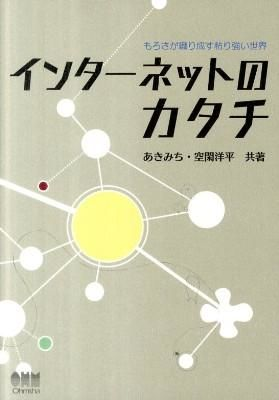
\includegraphics[width=70pt]{figures/katachi.jpg}\\
        
\includegraphics[width=70pt]{figures/v6plus.png}
      \end{column}
      \begin{column}[t]{0.3\textwidth}
      \centering
        
\includegraphics[width=70pt]{figures/openflow.jpg}\\
        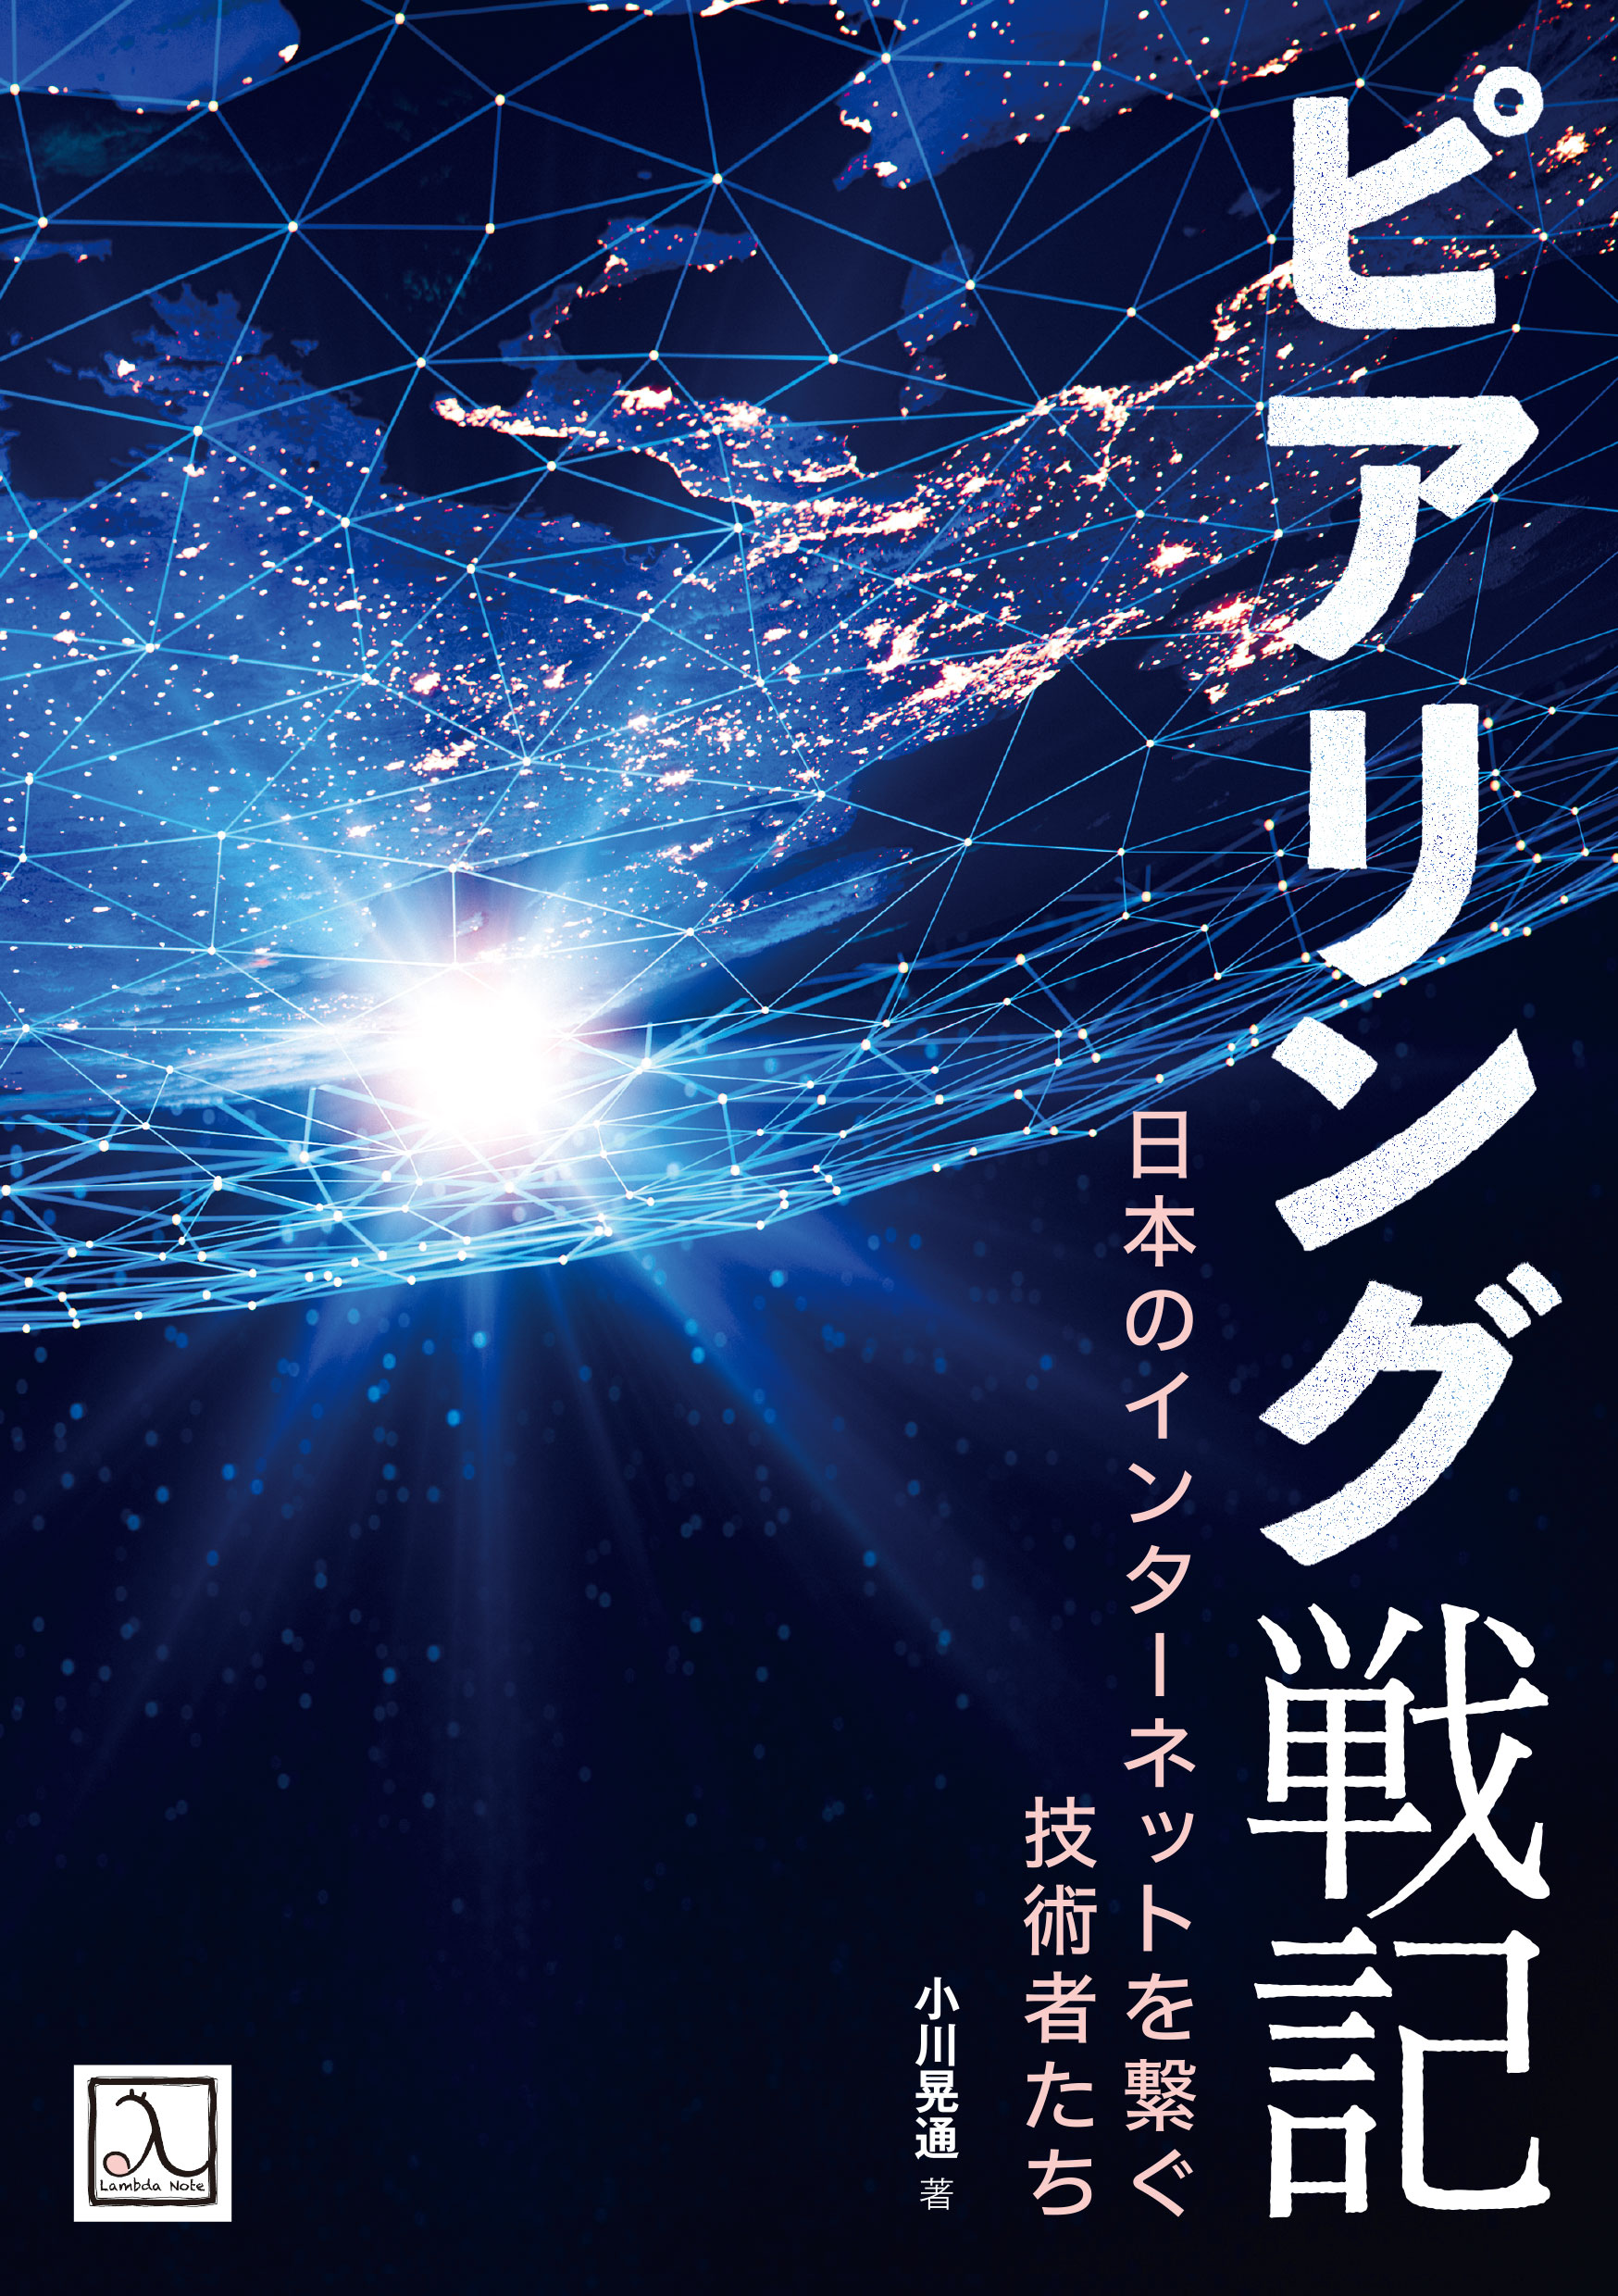
\includegraphics[width=70pt]{figures/peering.jpg}
      \end{column}
    \end{columns}

  \end{center}
\end{frame}


{\usebackgroundtemplate{%
  \begin{tikzpicture}[remember picture, overlay]
    \node[opacity=0.2,inner sep=0pt,yshift=-10pt] at (current page.center)
      {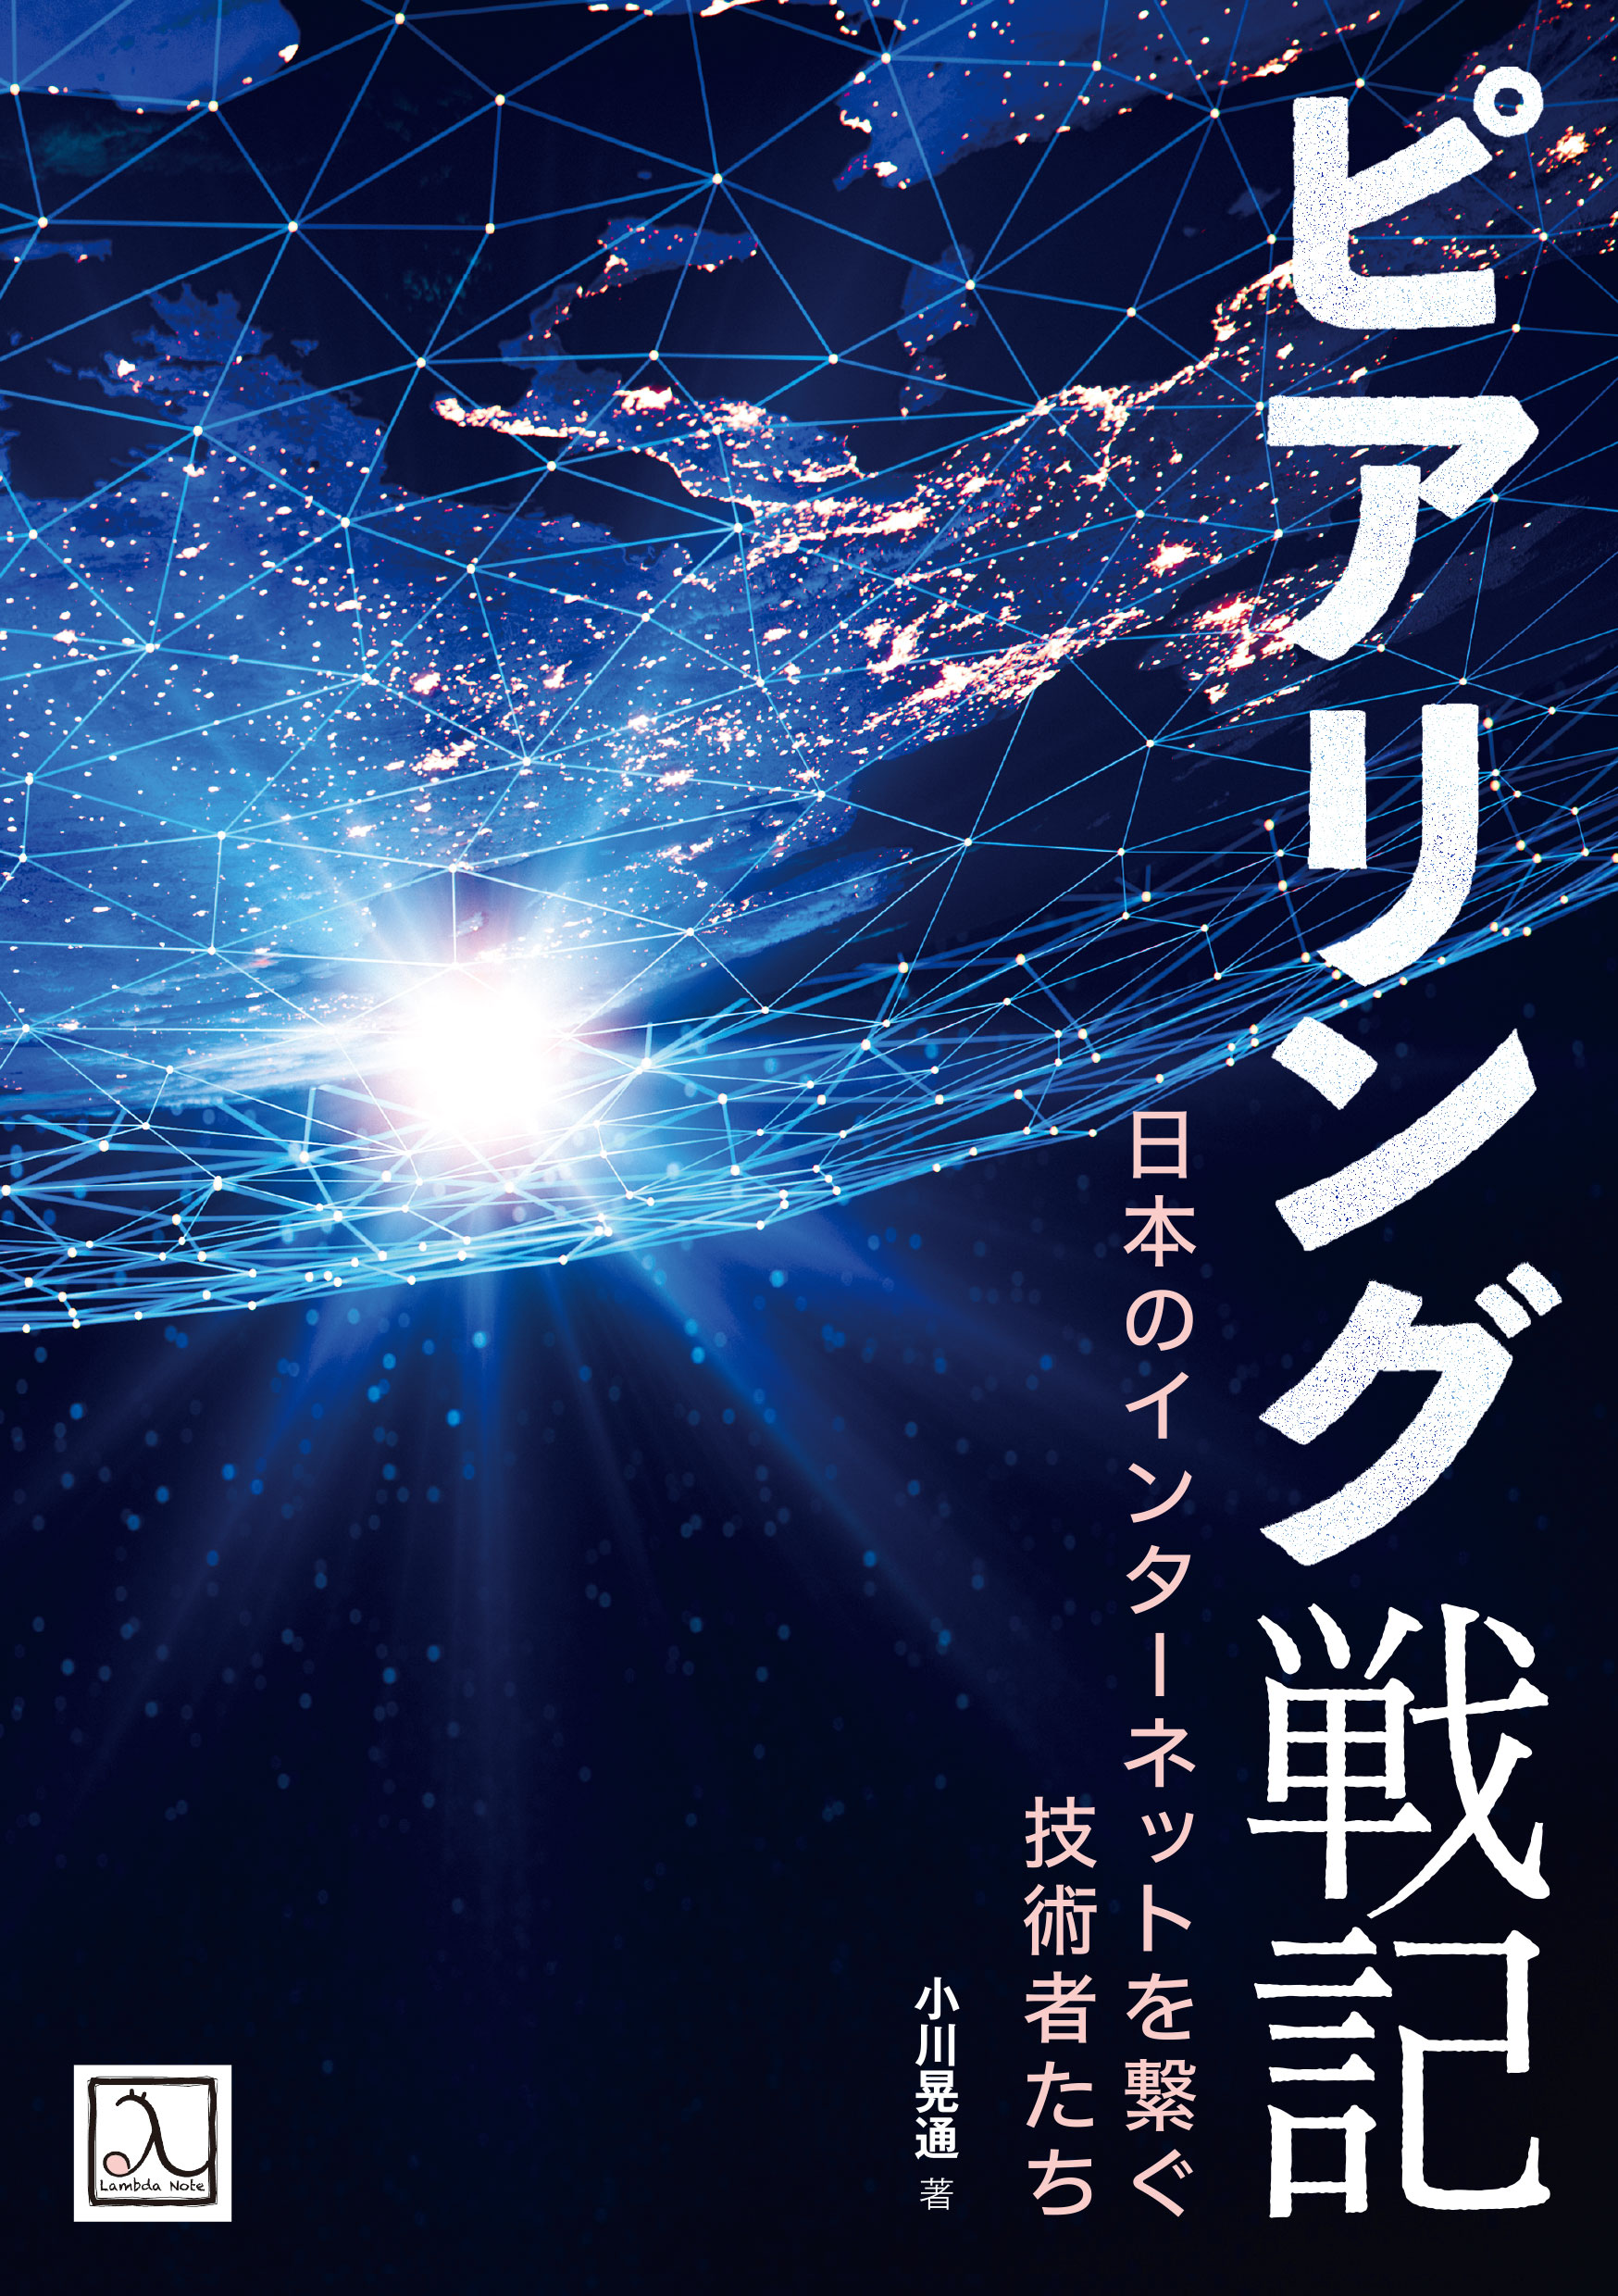
\includegraphics[height=180pt]{figures/peering.jpg}};
  \end{tikzpicture}}
\begin{frame}[plain]
  \begin{center}
    \HUGE{23}{23}\color{kachi}\yasagoth
    \bw{突然ですがクーポンのお知らせ}
    
    \bw{{\HUGE{19}{19}『ピアリング戦記』PDF版が20\%オフ!}}

    \bw{{\HUGE{15}{15}クーポンコード}}
    
    \bw{\HUGE{25}{25}「シンカンオマチランド」}
    
    \includegraphics[width=3\baselineskip]{figures/qrcode_202209221925.png}
    
    \bw{\HUGE{12}{12}\myurl{https://www.lambdanote.com/products/peering-ebook}}
    
    \bw{\HUGE{15}{15}期間限定 2022/9/23 ~ 9/25 まで}
    
  \end{center}
\end{frame}}


\setbeamertemplate{itemize item}{§}
\setbeamertemplate{itemize subitem}{$-$}
\setbeamercolor{itemize/enumerate body}{fg=kachi!70}
\setbeamercolor{itemize/enumerate subbody}{fg=black}
\setbeamerfont{itemize/enumerate body}{size={\fontsize{10}{10}}, family=\yasagoth}
\setbeamerfont{itemize/enumerate subbody}{size={\fontsize{13}{14}}, family=\sffamily}
\setbeamerfont{itemize/enumerate subsubbody}{size={\fontsize{12}{12}}, family=\sffamily}

{\usebackgroundtemplate{%
  \begin{tikzpicture}[remember picture, overlay]
    \node[opacity=0.3,inner sep=0pt,yshift=-10pt] at (current page.center)
      {
\includegraphics[height=180pt]{figures/rtp.jpg}};
  \end{tikzpicture}}
\begin{frame}{『マスタリングTCP/IP RTP編』}
\protect\hypertarget{ux30deux30b9ux30bfux30eaux30f3ux30b0tcpip-rtpux7de8}{}
\begin{itemize}
\tightlist
\item
  基本情報

  \begin{itemize}
  \tightlist
  \item
    \bw{Colin Perkins 著、小川 晃通 監訳}
  \item
    \bw{2004年4月、オーム社}
  \item
    \bw{\texttt{\small\url{https://www.ohmsha.co.jp/book/9784274065613/}}}
  \end{itemize}
\item
  企画の背景と発端

  \begin{itemize}
  \tightlist
  \item
    \bw{鹿野(出版社の編集者)が、翻訳の版権を獲得}
  \item
    「RTPに\bw{詳しそうな人」を探して、あきみちさんに連絡}
  \end{itemize}
\item
  制作技術

  \begin{itemize}
  \tightlist
  \item
    \bw{喫茶店で打ち合せしたり、休日に来社してもらったり、}ふつうの商業出版
  \item
    業者による翻訳 \bw{→ 版元で翻訳チェックと仮組版 → 監訳}
  \end{itemize}
\end{itemize}
\end{frame}}

{\usebackgroundtemplate{%
  \begin{tikzpicture}[remember picture, overlay]
    \node[opacity=0.3,inner sep=0pt,yshift=-10pt] at (current page.center)
      {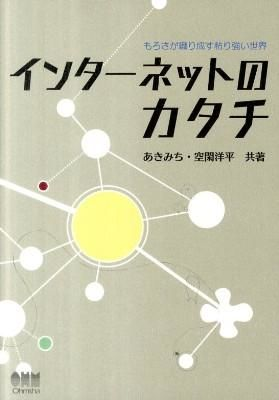
\includegraphics[height=180pt]{figures/katachi.jpg}};
  \end{tikzpicture}}
\begin{frame}{『インターネットのカタチ』}
\protect\hypertarget{ux30a4ux30f3ux30bfux30fcux30cdux30c3ux30c8ux306eux30abux30bfux30c1}{}
\begin{itemize}
\tightlist
\item
  基本情報

  \begin{itemize}
  \tightlist
  \item
    \bw{あきみち 著、空閑 洋平 著}
  \item
    \bw{2011年6月、オーム社}
  \item
    \bw{\texttt{\small\url{https://www.ohmsha.co.jp/book/9784274068249/}}}
  \end{itemize}
\item
  企画の背景と発端

  \begin{itemize}
  \tightlist
  \item
    \bw{あきみちさんがブロガー @geekpage として独立}
  \item
    「インターネットが\bw{壊れた話のネタがいろいろある」}といって持ち込み
  \end{itemize}
\item
  制作技術

  \begin{itemize}
  \tightlist
  \item
    \bw{TeXで執筆、Subversionのリモートサーバで}バージョン管理
  \end{itemize}
\end{itemize}
\end{frame}}

{\usebackgroundtemplate{%
  \begin{tikzpicture}[remember picture, overlay]
    \node[opacity=0.3,inner sep=0pt,yshift=-10pt] at (current page.center)
      {
\includegraphics[height=180pt]{figures/openflow.jpg}};
  \end{tikzpicture}}
\begin{frame}{『マスタリングTCP/IP OpenFlow編』}
\protect\hypertarget{ux30deux30b9ux30bfux30eaux30f3ux30b0tcpip-openflowux7de8}{}
\begin{itemize}
\tightlist
\item
  基本情報

  \begin{itemize}
  \tightlist
  \item
    \bw{あきみち 著、宮永 直樹 著、岩田 淳 著}
  \item
    \bw{2013年7月、オーム社}
  \item
    \bw{\texttt{\small\url{https://www.ohmsha.co.jp/book/9784274069208/}}}
  \end{itemize}
\item
  企画の背景と発端

  \begin{itemize}
  \tightlist
  \item
    \bw{鹿野がSDNに興味を持って、あきみちさんと雑談してた}のがきっかけ
  \end{itemize}
\item
  制作技術

  \begin{itemize}
  \tightlist
  \item
    \bw{HTMLで執筆、Subversionのリモートサーバ}でバージョン管理
  \item
    \bw{自動組版システム(Scheme+LaTeX)}
  \end{itemize}
\end{itemize}
\end{frame}}

{\usebackgroundtemplate{%
  \begin{tikzpicture}[remember picture, overlay]
    \node[opacity=0.3,inner sep=0pt,yshift=-10pt] at (current page.center)
      {
\includegraphics[height=180pt]{figures/ipv6.png}};
  \end{tikzpicture}}
\begin{frame}{『プロフェッショナルIPv6』}
\protect\hypertarget{ux30d7ux30edux30d5ux30a7ux30c3ux30b7ux30e7ux30caux30ebipv6}{}
\begin{itemize}
\tightlist
\item
  基本情報

  \begin{itemize}
  \tightlist
  \item
    小川 晃通 著
  \item
    \bw{2018年7月、ラムダノート}
  \item
    \bw{\texttt{\small\url{https://lambdanote.com/products/ipv6}}}
  \end{itemize}
\item
  企画の背景と発端

  \begin{itemize}
  \tightlist
  \item
    鹿野が出版社 \bw{@lambdanote として独立}
  \item
    「完成してない\bw{原稿をなんとかしたい」が、}印税収入だと厳しい

    \begin{itemize}
    \tightlist
    \item
      「もう\bw{本は書かないで」}
    \end{itemize}
  \item
    \bw{クラウドファンディングでの出版に挑戦してみよう}
  \end{itemize}
\item
  制作技術

  \begin{itemize}
  \tightlist
  \item
    \bw{HTMLで執筆、GitHubでバージョン管理}
  \item
    自動組版システム(Scheme+LaTeX)
  \end{itemize}
\end{itemize}
\end{frame}}

{\usebackgroundtemplate{%
  \begin{tikzpicture}[remember picture, overlay]
    \node[opacity=0.3,inner sep=0pt,yshift=-10pt] at (current page.center)
      {
\includegraphics[height=180pt]{figures/v6plus.png}};
  \end{tikzpicture}}
\begin{frame}{『徹底解説 v6プラス』}
\protect\hypertarget{ux5fb9ux5e95ux89e3ux8aacv6ux30d7ux30e9ux30b9}{}
\begin{itemize}
\tightlist
\item
  基本情報

  \begin{itemize}
  \tightlist
  \item
    \bw{日本ネットワークイネイブラー株式会社 監修、小川 晃通}・久保田 聡 共著
  \item
    \bw{2020年1月、ラムダノート}
  \item
    \bw{\texttt{\small\url{https://lambdanote.com/products/v6plus}}}
  \end{itemize}
\item
  企画の背景と発端

  \begin{itemize}
  \tightlist
  \item
    『プロ\bw{フェッショナルIPv6』のスポンサー}でもあるJPNEさんから、\bw{あきみちさんに打診}
  \item
    \bw{サービスマニュアルやマーケ資料としてでなく}、あくまでも「技術書」\bw{として企画}

    \begin{itemize}
    \tightlist
    \item
      \bw{大規模NAT技術について詳しい稀有な本に}
    \end{itemize}
  \end{itemize}
\item
  制作技術

  \begin{itemize}
  \tightlist
  \item
    \bw{Markdownで執筆、GitHubでバージョン管理}
  \item
    自動組版システム(Haskell+LaTeX)
  \end{itemize}
\end{itemize}
\end{frame}}

{\usebackgroundtemplate{%
  \begin{tikzpicture}[remember picture, overlay]
    \node[opacity=0.3,inner sep=0pt,yshift=-10pt] at (current page.center)
      {
\includegraphics[height=180pt]{figures/ipv6-2.jpg}};
  \end{tikzpicture}}
\begin{frame}{『プロフェッショナルIPv6 第2版』}
\protect\hypertarget{ux30d7ux30edux30d5ux30a7ux30c3ux30b7ux30e7ux30caux30ebipv6-ux7b2c2ux7248}{}
\begin{itemize}
\tightlist
\item
  基本情報

  \begin{itemize}
  \tightlist
  \item
    \bw{小川 晃通 著}
  \item
    \bw{2021年12月、ラムダノート}
  \item
    \bw{\texttt{\small\url{https://lambdanote.com/products/ipv6-2}}}
  \end{itemize}
\end{itemize}

  \vskip\baselineskip
  
  \bw{追加のクラウドファンディングも企業スポンサーもなしで改訂に成功}
\end{frame}}

{\usebackgroundtemplate{%
  \begin{tikzpicture}[remember picture, overlay]
    \node[opacity=0.2,inner sep=0pt,yshift=-10pt] at (current page.center)
      {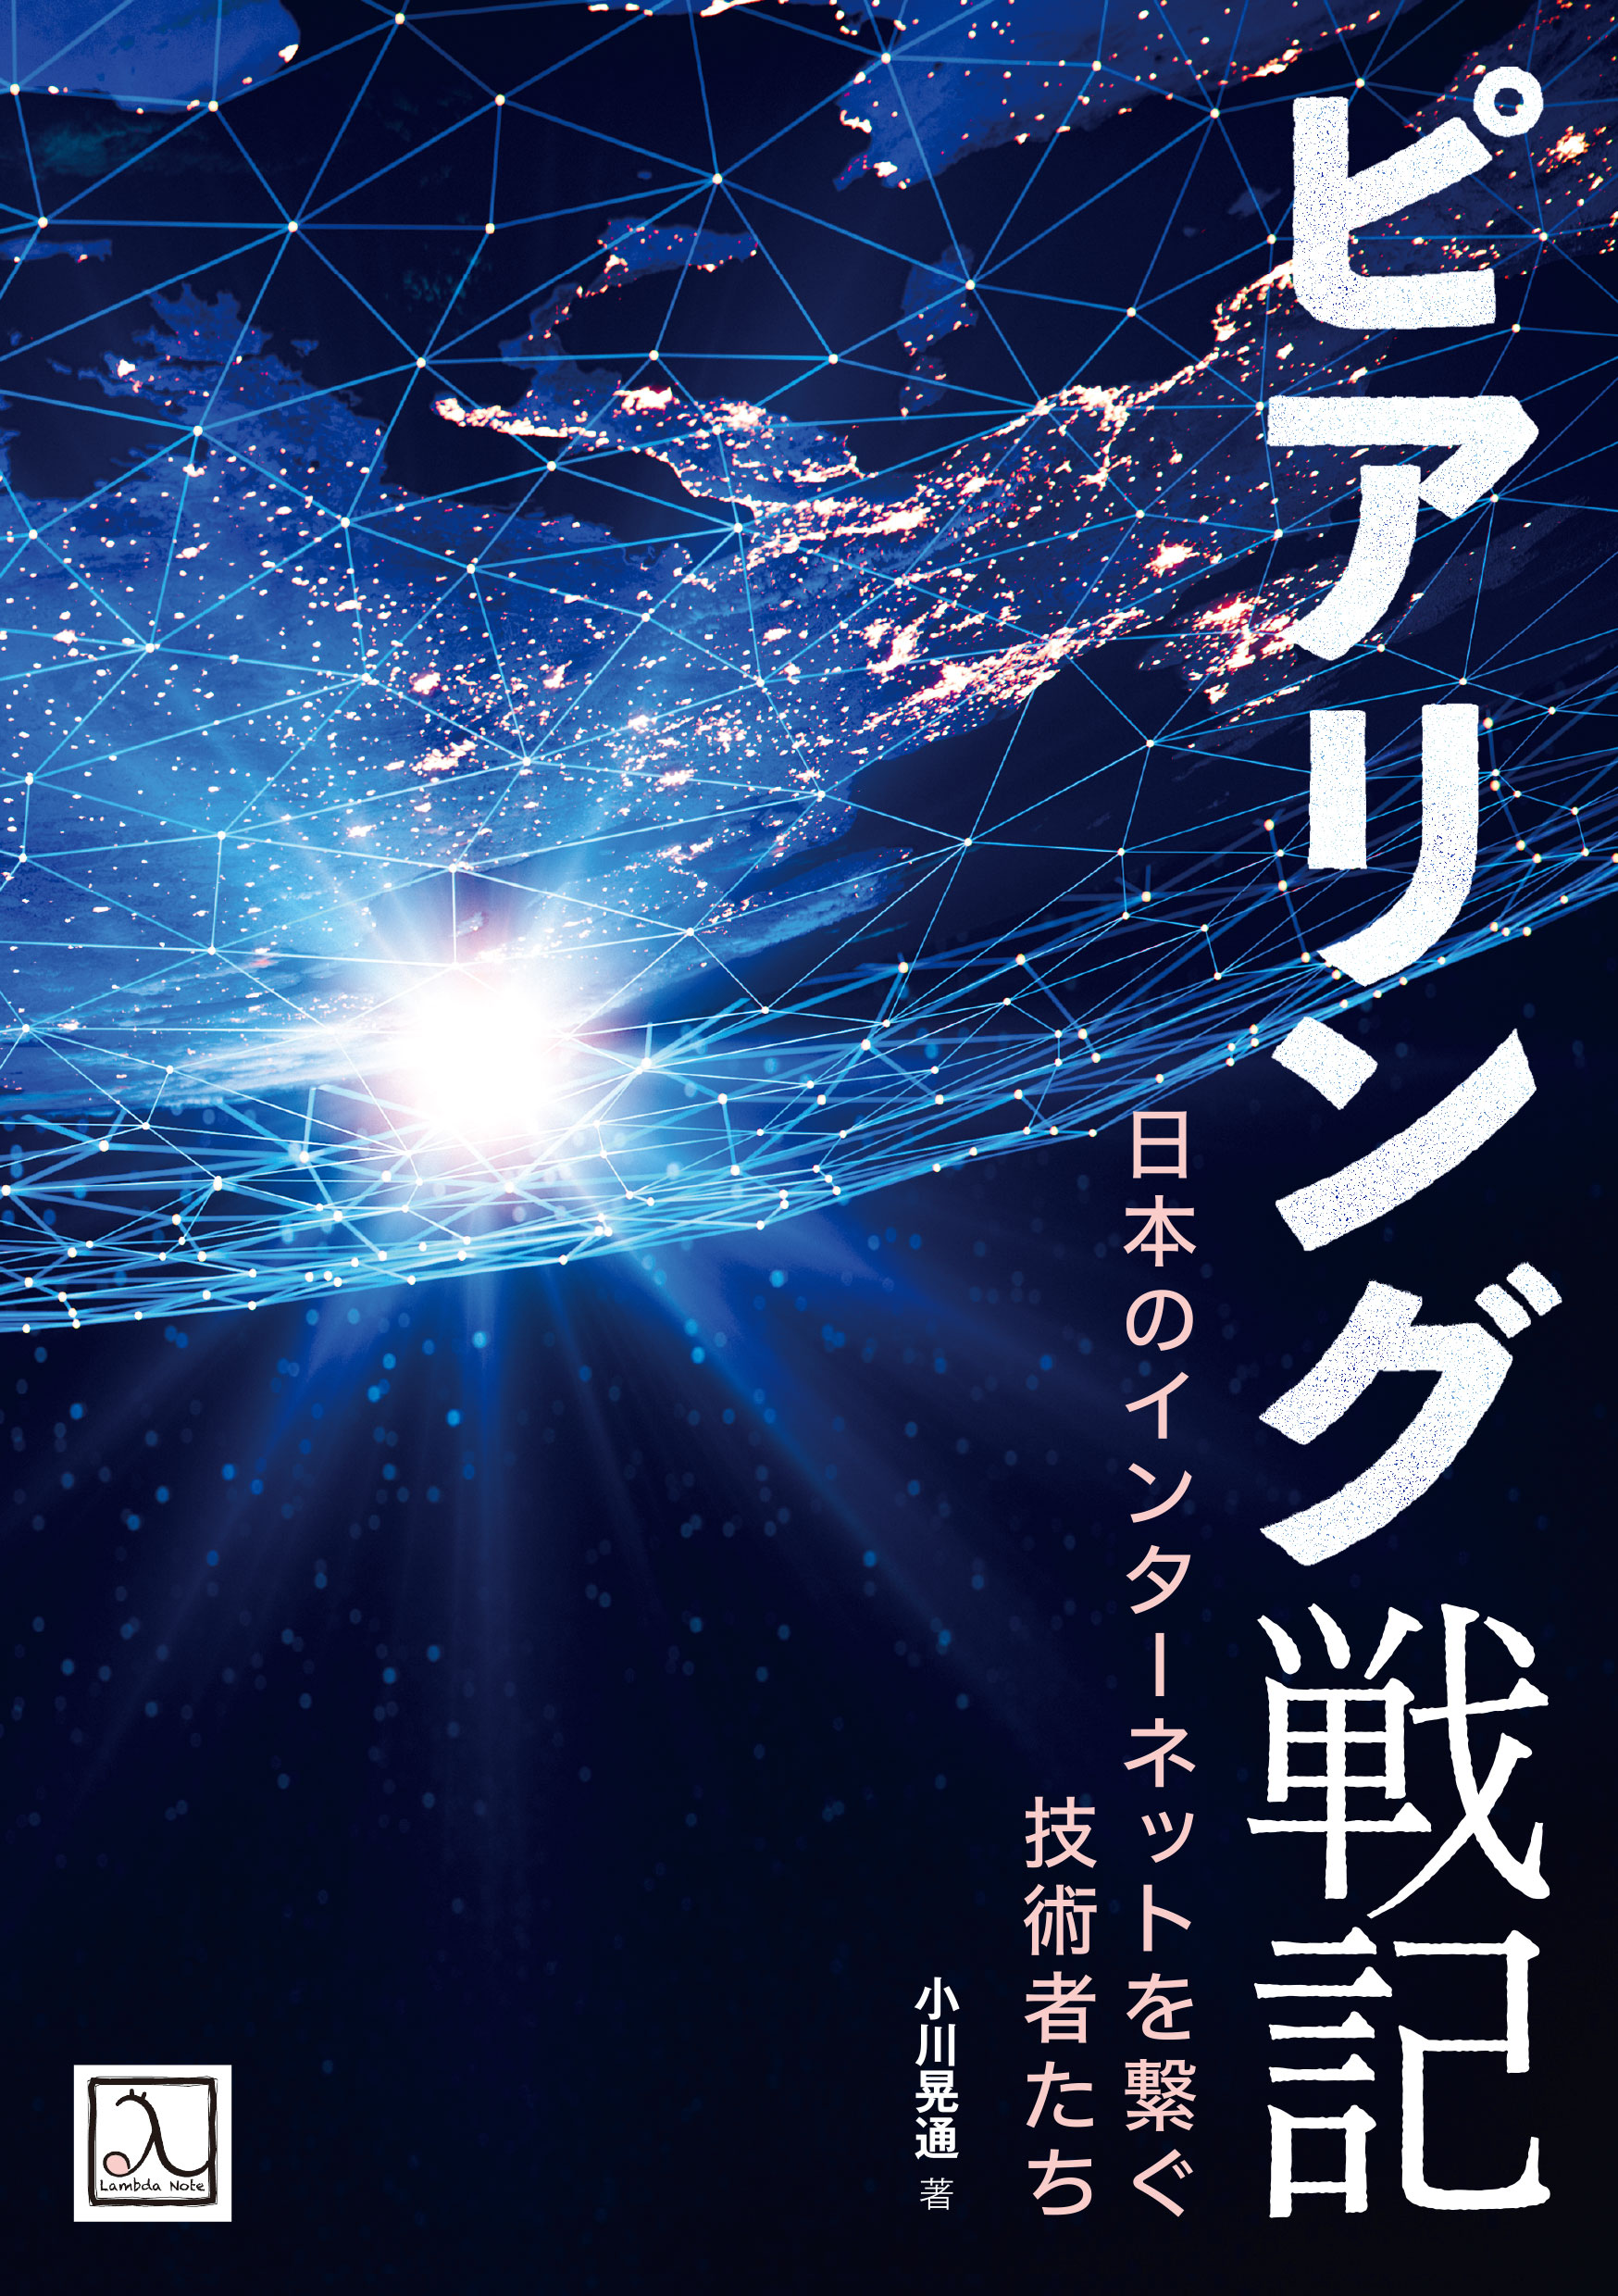
\includegraphics[height=180pt]{figures/peering.jpg}};
  \end{tikzpicture}}
\begin{frame}{『ピアリング戦記』}
\protect\hypertarget{ux30d4ux30a2ux30eaux30f3ux30b0ux6226ux8a18}{}
\begin{itemize}
\tightlist
\item
  基本情報

  \begin{itemize}
  \tightlist
  \item
    小川 晃通 著
  \item
    2022年7月、\bw{ラムダノート}
  \item
    \bw{\texttt{\small\url{https://lambdanote.com/products/peering}}}
  \end{itemize}
\item
  企画の背景と発端

  \begin{itemize}
  \tightlist
  \item
    ピアリング技術\bw{のコミュニティの中の方々}(発起人)から、\bw{あきみちさんに打診}
  \item
    どういう本が\bw{できるかわからないけど、とりあえず}当時を知っている\bw{人たちに順番に話を聞こう}
  \item
    「本」として\bw{まとまるまでは、あきみちさん}も鹿野もそれぞれ苦労した
  \end{itemize}
\item
  制作技術

  \begin{itemize}
  \tightlist
  \item
    \bw{Markdownで執筆、GitHubでバージョン管理}
  \item
    自動組版システム(Haskell+LaTeX)
  \end{itemize}
\end{itemize}
\end{frame}}


\setbeamertemplate{itemize items}[circle]
\setbeamercolor{itemize/enumerate body}{fg=black}
\setbeamercolor{itemize/enumerate subbody}{fg=kachi!70}
\setbeamerfont{itemize/enumerate body}{size={\fontsize{13}{14}}, family=\yasagoth}
\setbeamerfont{itemize/enumerate subbody}{size={\fontsize{12}{13}}, family=\sffamily}
\setbeamerfont{itemize/enumerate subsubbody}{size={\fontsize{12}{12}}, family=\sffamily}

\begin{frame}{よく考えること(本の内容以外)}
\protect\hypertarget{ux30b3ux30f3ux30c6ux30f3ux30c4ux306eux3053ux3068ux4ee5ux5916ux306bux3069ux3093ux306aux3053ux3068ux3092ux8003ux3048ux3066ux3044ux308bux304b}{}
\begin{itemize}
\tightlist
\item
  基本は「書きたいことがある →
  本にする」だけど、本で生計を立てているとそうもいかない

  \begin{itemize}
  \tightlist
  \item
    クラウドファンディング
  \item
    企業/個人スポンサー
  \item
    フリーミアム
  \end{itemize}
\item
  出版には責任も伴う

  \begin{itemize}
  \tightlist
  \item
    間違いがない内容にすることは前提
  \item
    無理に買わせない
  \item
    パッケージ化された情報として残すことの意義
  \end{itemize}
\item
  バージョン管理と自動組版は空気と水のようなもの
\end{itemize}
\end{frame}

\begin{frame}[plain]
  \begin{center}
    \HUGE{34}{34}\color{kachi}\yasagoth
    QA
  \end{center}
\end{frame}

\end{document}